\problemname{Finding Clusters
}

\intextsep2mm
\begin{wrapfigure}{r}{50mm}
 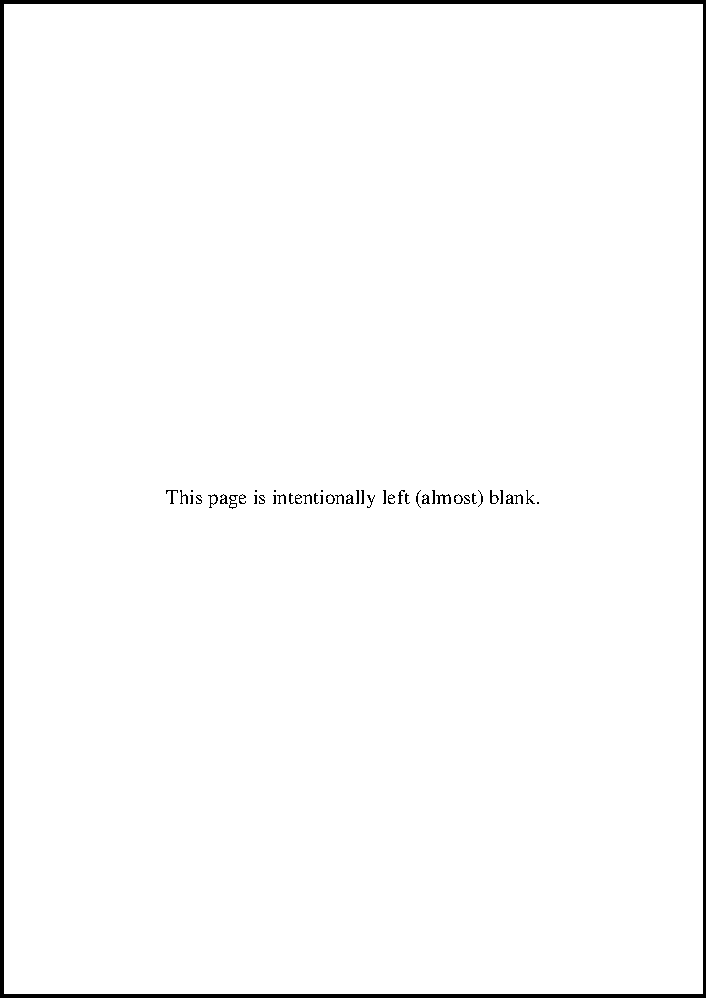
\includegraphics[width=50mm]{img.pdf}
\end{wrapfigure}
~

You just came up with the brilliant PageBlank algorithm, which drastically improves the quality of web search results.
To avoid manipulation, it needs to detect and analyse artificial, highly interlinked clusters of web pages.

The web is modelled as a set of $n$ web pages with links between them. A non-empty set $S$ of web pages is a \textit{cluster} if for every page $p$ in the web (not just for the web pages in $S$), $p$ is in the set $S$ if and only if there is a page $q$ in the set $S$ such that $q$ contains a link to $p$.

Two clusters can be compared to determine which is more suspicious. Given two clusters $S$ and $T$, let $p$ be the smallest identifier in exactly one of $S$ and $T$.
If $p$ is in $S$ but not in $T$, then $T$ is more suspicious; otherwise, $S$ is more suspicious.

Out of all clusters, which is the most suspicious?



\section*{Input}

The first line of the input contains a single integer $n$~($1 \leq n \leq 10^5$), which is the number of web pages.

Each of the next $n$ lines describes the links contained in a web page.
Each line starts with the number of links $m_i$ ($1 \leq m_i \leq 10^6$), followed by $m_i$ distinct integers $a_{ij}$ in ascending order, which are the linked web pages ($1 \leq a_{ij} \leq n$).
Web pages are numbered from $1$ to $n$ in the order they are described in the input.
The total number of links is at most $10^6$.


\section*{Output}

Display the web pages in the most suspicious cluster. List these pages using their identifiers in ascending order. It can be proven that at least one cluster exists given the constraints for the problem.


